\documentclass{article}

% if you need to pass options to natbib, use, e.g.:
%     \PassOptionsToPackage{numbers, compress}{natbib}
% before loading neurips_2026


% The authors should use one of these tracks.
% Before accepting by the NeurIPS conference, select one of the options below.
% "default" for submission

% this is comment

\usepackage{neurips_2026_vericode}

% After being accepted, the authors should add "final" behind the track to compile a camera-ready version.
% \usepackage[main, final]{neurips_2026_vericode}

% "preprint" option is used for arXiv or other preprint submissions
 % \usepackage[preprint]{neurips_2026_vericode}

% to avoid loading the natbib package, add option nonatbib:
%    \usepackage[nonatbib]{neurips_2026_vericode}

\usepackage[utf8]{inputenc} % allow utf-8 input
\usepackage[T1]{fontenc}    % use 8-bit T1 fonts
\usepackage{hyperref}       % hyperlinks
\usepackage{graphicx} 
\usepackage{float}          % [H] to pin figures in place
\graphicspath{{main-results/figures/}}
\usepackage{url}            % simple URL typesetting
\usepackage{booktabs}       % professional-quality tables
\usepackage{amsfonts}       % blackboard math symbols
\usepackage{nicefrac}       % compact symbols for 1/2, etc.
\usepackage{microtype}      % microtypography
\usepackage{xcolor}         % colors

% Note. For the workshop paper template, both \title{} and \workshoptitle{} are required, with the former indicating the paper title shown in the title and the latter indicating the workshop title displayed in the footnote. 
\title{Deterministically Measuring Autoformalization Faithfulness}


% The \author macro works with any number of authors. There are two commands
% used to separate the names and addresses of multiple authors: \And and \AND.
%
% Using \And between authors leaves it to LaTeX to determine where to break the
% lines. Using \AND forces a line break at that point. So, if LaTeX puts 3 of 4
% authors names on the first line, and the last on the second line, try using
% \AND instead of \And before the third author name.

\newcommand{\shivam}[1]{\textcolor{magenta}{(Shivam: #1)}}

\newcommand{\oren}[1]{\textcolor{teal}{(Oren: #1)}}

\newcommand{\denis}[1]{\textcolor{red}{(Denis: #1)}}

\newcommand{\harsh}[1]{\textcolor{olive}{(Harsh: #1)}}

\newcommand{\Ke}[1]{\textcolor{blue}{(Ke: #1)}}

\newcommand{\aditya}[1]{\textcolor{orange}{(aditya: #1)}}


\author{%
  David S.~Hippocampus\thanks{Use footnote for providing further information
    about author (webpage, alternative address)---\emph{not} for acknowledging
    funding agencies.} \\
  Department of Computer Science\\
  Cranberry-Lemon University\\
  Pittsburgh, PA 15213 \\
  \texttt{hippo@cs.cranberry-lemon.edu} \\
  % examples of more authors
  % \And
  % Coauthor \\
  % Affiliation \\
  % Address \\
  % \texttt{email} \\
  % \AND
  % Coauthor \\
  % Affiliation \\
  % Address \\
  % \texttt{email} \\
  % \And
  % Coauthor \\
  % Affiliation \\
  % Address \\
  % \texttt{email} \\
  % \And
  % Coauthor \\
  % Affiliation \\
  % Address \\
  % \texttt{email} \\
}


\begin{document}

632960
\maketitle


\begin{abstract}
  Autoformalization with LLMs can enable proofs, programs, and AI-generated claims to be verified at a scale no human reviewer could match. Yet verifying the faithfulness of these formalizations without a human judge remains a challenge. We introduce a  benchmark for measuring formalization faithfulness. By deterministically rendering magma equations from the Equational Theories Project into natural-language stories that capture the same logical meaning, we obtain formal-informal pairs that are correct by construction and generated at scale. Models are then asked to recover the equation underlying each story. Evaluating nine models with reasoning disabled, we find that they achieve 50\% accuracy on story translations. We further show that decomposing the formalization task into a two-stage pipeline, where a model first abstracts the story into a bare logical statement before formalizing it, increases accuracy by 16\%. Enabling inference-time reasoning increases accuracy to 100\% for stories generated from simple equations with few magma operations, but this accuracy degrades to approximately 75\% as complexity increases.
\end{abstract}


\section{Introduction}

Autoformalization translates informal natural-language statements into formal specifications that can be processed by theorem provers and other automated
reasoning systems~\citep{wu2022autoformalization}. Its usefulness depends not only on producing syntactically valid or provable statements, but also on preserving the meaning of the source. A formal statement may admit a proof while expressing a different claim. A proof checker cannot
detect this mismatch because it verifies the generated statement rather than its correspondence to the intended natural-language meaning ~\citep{kim2026gaming}. We refer to such a mismatch as \textit{semantic drift}.

Semantic drift can occur in several ways. A model tasked with autoformalizing may misunderstand the logical content of the source, or it may understand that
 content but fail to express it in the target formalism. In a system such as Lean ~\citep{demoura2021lean4}, formalizing requires knowledge of syntax, types, elaboration, and library conventions. These requirements make it difficult to tell whether an observed failure comes from source interpretation, target
encoding, or the faithfulness metric itself.

Detecting semantic drift is difficult. Human evaluation is expensive, while language-model judges can accept incorrect formalizations or reject correct
ones~\citep{kimina2025,chen2025reform}. Proof-based equivalence checks require a trusted reference formalization and may still depend on incomplete proof
search. \aditya{this claim requires a citation} As a result, existing evaluations often lack a scalable and deterministic way to determine whether the meaning of a source statement has been preserved.



We construct a benchmark using implications from the Equational Theories Project (ETP)~\citep{bolan2025etp}, each of which states that one equation over a binary operation implies another. Each statement is rendered
deterministically in two matched forms: \textit{Story}, which reimagines the equation as a natural-language narrative involving real-world objects and actions, and \textit{Literal-NL}, which
describes the same operation structure directly in natural language without the narrative framing. We ask models to translate each description into a
minimal, mechanically parseable grammar.

The benchmark allows us to study different parts of the translation process. Translating from Story tests the model's ability to
recover the same logical structure from a narrative. Translating from Literal-NL provides a control for the
remaining target-encoding difficulty. We  also evaluate a two-stage pipeline in which the model is tasked to first remove the narrative flourish and then
formalize the resulting abstraction. Together, these conditions let us ask
how source presentation, explicit decomposition, reasoning, and structural
complexity affect semantic preservation.

Across nine models evaluated without reasoning on the same 160 ETP pairs,
translating from Story achieves 50\% accuracy, compared with 67\% for
Literal-NL. The two-stage pipeline reaches 66\%, recovering most of the gap
between the two source forms. With reasoning enabled, performance rises to
97\% for Story, 99\% for Literal-NL, and 96\% for the two-stage protocol.
These results indicate that narrative abstraction creates a measurable
translation cost, but that explicit decomposition or additional
inference-time reasoning can substantially reduce it.

Our main contributions are:

\begin{itemize}
    \item We introduce a controlled benchmark in which semantic preservation
    can be graded deterministically against a retained formal source, without
    relying on a human or language-model judge.

    \item We use paired Story and Literal-NL renderings with a shared minimal
    target grammar to distinguish the additional difficulty of narrative
    abstraction from target encoding.

    \item We evaluate how explicit two-stage abstraction, reasoning, and
    structural complexity affect faithful recovery of the underlying formal
    statement.
\end{itemize}

Our benchmark does not provide a general metric for arbitrary
natural-language mathematics. Instead, it provides a controlled setting in
which semantic mismatch is directly observable and factors that contribute to
it can be studied separately. This offers a foundation for investigating how
the same distinctions extend to richer natural language and practical formal
systems.


%\subsubsection{Background}
%Formalization is the process of capturing the logical meaning of a natural-language statement in a formal language: one with a rigid grammar and a fixed semantics. For mathematics and logic, the value of formalization lies in what it makes possible afterward. Once a problem has been stated formally, a proposed solution can be checked mechanically by the kernel of a proof assistant such as Lean [cite], a small trusted program that only accepts correct proofs. This is what allows large collaborative results to be trusted without any single participant checking the whole [cite], and it is what makes formal languages the natural target for automated reasoning systems, since a machine-checked proof needs no further review.


%, and few people have both. Formalizing even a routine statement requires fluency in both the mathematics and the formal system \textit{Autoformalization}, the automatic translation of informal mathematics into formal statements, now typically performed by a large language model, has accordingly attracted wide interest [cite]. 




\section{Related works}

\shivam{the related works needs rewrite, I'll have to think about what bifurcation makes sense but it needs to be one level of abstraction higher. So something like 1. Autoformalization for scalable oversight: {all papers that are not directly related to our work but broadly supporting our motivation} 2.Faithfulness problem in autoformalization 3. something around semantic parsing}

\oren{ I don't think Scalable Oversight should have a section in Related Works because our methods do not specifically target scalable oversight. I think the scalable oversight motivation should remain in the introduction}

\paragraph{Informalization for data generation}
The strongest current autoformalizers are language models fine-tuned on formal-informal pairs.~\citep{gao2025herald,kimina2025,lin2025goedel}. Oftentimes, their training data is manufactured by having an LLM informalize an existing formal library.~\citep{jiang2023mma,gao2025herald,ying2024leanworkbook,xin2024deepseekprover}. We use informalization for the opposite purpose: performed by a deterministic renderer rather than a model, it yields an evaluation oracle instead of training data. This enables an exact ground truth formalization.  

\paragraph{Measuring faithfulness.}
Human-labelled sets such as ProofNetVerif~\citep{poiroux2025reliable}, ConsistencyCheck~\citep{chen2025reform}, CriticLeanBench~\citep{criticlean2025}, and MA-Align~\citep{mathatlas2026} are expensive to build, and the references they rest on are themselves unreliable: annotation found 16.4\% of the human-written formal statements in miniF2F and 38.5\% of those in ProofNet to be semantically wrong~\citep{chen2025reform}. Model-based methods trust a language model as a judge~\citep{ying2024leanworkbook,lin2025goedel,kimina2025}, a trained critic~\citep{lu2025formalalign,criticlean2025,mathesis2025}, or a back-translator~\citep{patel2024newsymbol,li2024symbolic}; the best judges agree with experts about 86\% of the time~\citep{chen2025reform}, and in specification autoformalization a judge missed a quarter of the failures that an executable check caught~\citep{verusspecgym2026}. Prover-based methods trust an automated prover to establish equivalence with a reference~\citep{liu2025rethinking,poiroux2025reliable,murphy2024leaneuclid,liu2025gted}, and so need both a reference and a proof search that may time out. Every method above needs a human, a model, or an incomplete prover somewhere in the loop. 
 
\paragraph{Synthetic language with exact ground truth.}
Synthetic and semi-synthetic reasoning benchmarks construct
natural-language problems from controlled underlying
structures~\citep{weston2015babi,sinha2019clutrr,clark2020ruletaker,tafjord2021proofwriter}.
ZebraLogic uses clue templates~\citep{zebralogic2025},
whereas SATBench uses LLMs (not deterministic) and tests solving, not translation~\citep{satbench2025}. FOLIO combines expert-written
and template-assisted stories and also evaluates
natural-language-to-first-order-logic translation~\citep{han2022folio}.
 
\paragraph{Staged formalization.}
Passing through an intermediate representation on the way to a formal target is an old idea in semantic parsing, whether a canonical utterance~\cite{shin2021constrained} or an intermediate query language~\cite{guo2019irnet,gan2021natsql}. Prompting methods that first abstract a problem~\cite{zheng2023stepback} or draft an informal sketch~\cite{jiang2023dsp} follow the same pattern, and formalize-then-solve pipelines identify translation as a major source of error~\cite{olausson2023linc,pan2023logiclm,ye2023satlm,lyu2023faithfulcot}, motivating decomposition of the translation step~\cite{ryu2024divide}. The remedies proposed for autoformalization add a verifier or a feedback loop: reflective refinement~\cite{chen2025reform}, faithfulness-guided decoding~\cite{mohammad2026faithfulness}, or reranking candidates by symbolic equivalence~\cite{li2024symbolic}. Our two-stage route uses neither. It changes only how the model is asked, and it composes with any of them.


\section{Constructing the Benchmark} 
Each benchmark item begins with an ordered pair $(E,F)$ of equational laws
from ETP, representing the claim that every binary operation satisfying $E$
also satisfies $F$. The benchmark asks a model to recover this formal claim
from one of its natural-language renderings. Figure~\ref{fig:pipeline} summarizes the following four
steps:

\begin{enumerate}
    \item \textbf{Sample and construct the reference.}
    We sample an ordered pair $(E,F)$ of ETP laws and retain its formal syntax
    trees as the ground-truth statement. The pair is serialized into the
    benchmark-specific Rigid Grammar, and the permitted symmetry
    transformations are enumerated to construct the set of acceptable answers.

    \item \textbf{Render the statement.}
    Deterministic renderers express the same pair in two matched forms:
    \textit{Story} and
    \textit{Literal-NL}. The model is never shown the
    original ETP equations.

    \item \textbf{Translate into Rigid Grammar.}
    The model receives one natural-language rendering, a self-contained
    definition of the target syntax, and a small set of worked examples. 
    \item \textbf{Parse and grade the translation.}
    The grader extracts and parses
    the model response and classifies it as \textit{correct} if it
    matches an accepted variant, \textit{wrong} if it is parseable but
    represents a different statement, and \textit{unparseable} if extraction
    or parsing fails.
\end{enumerate}

\begin{figure}[t]
  \centering
  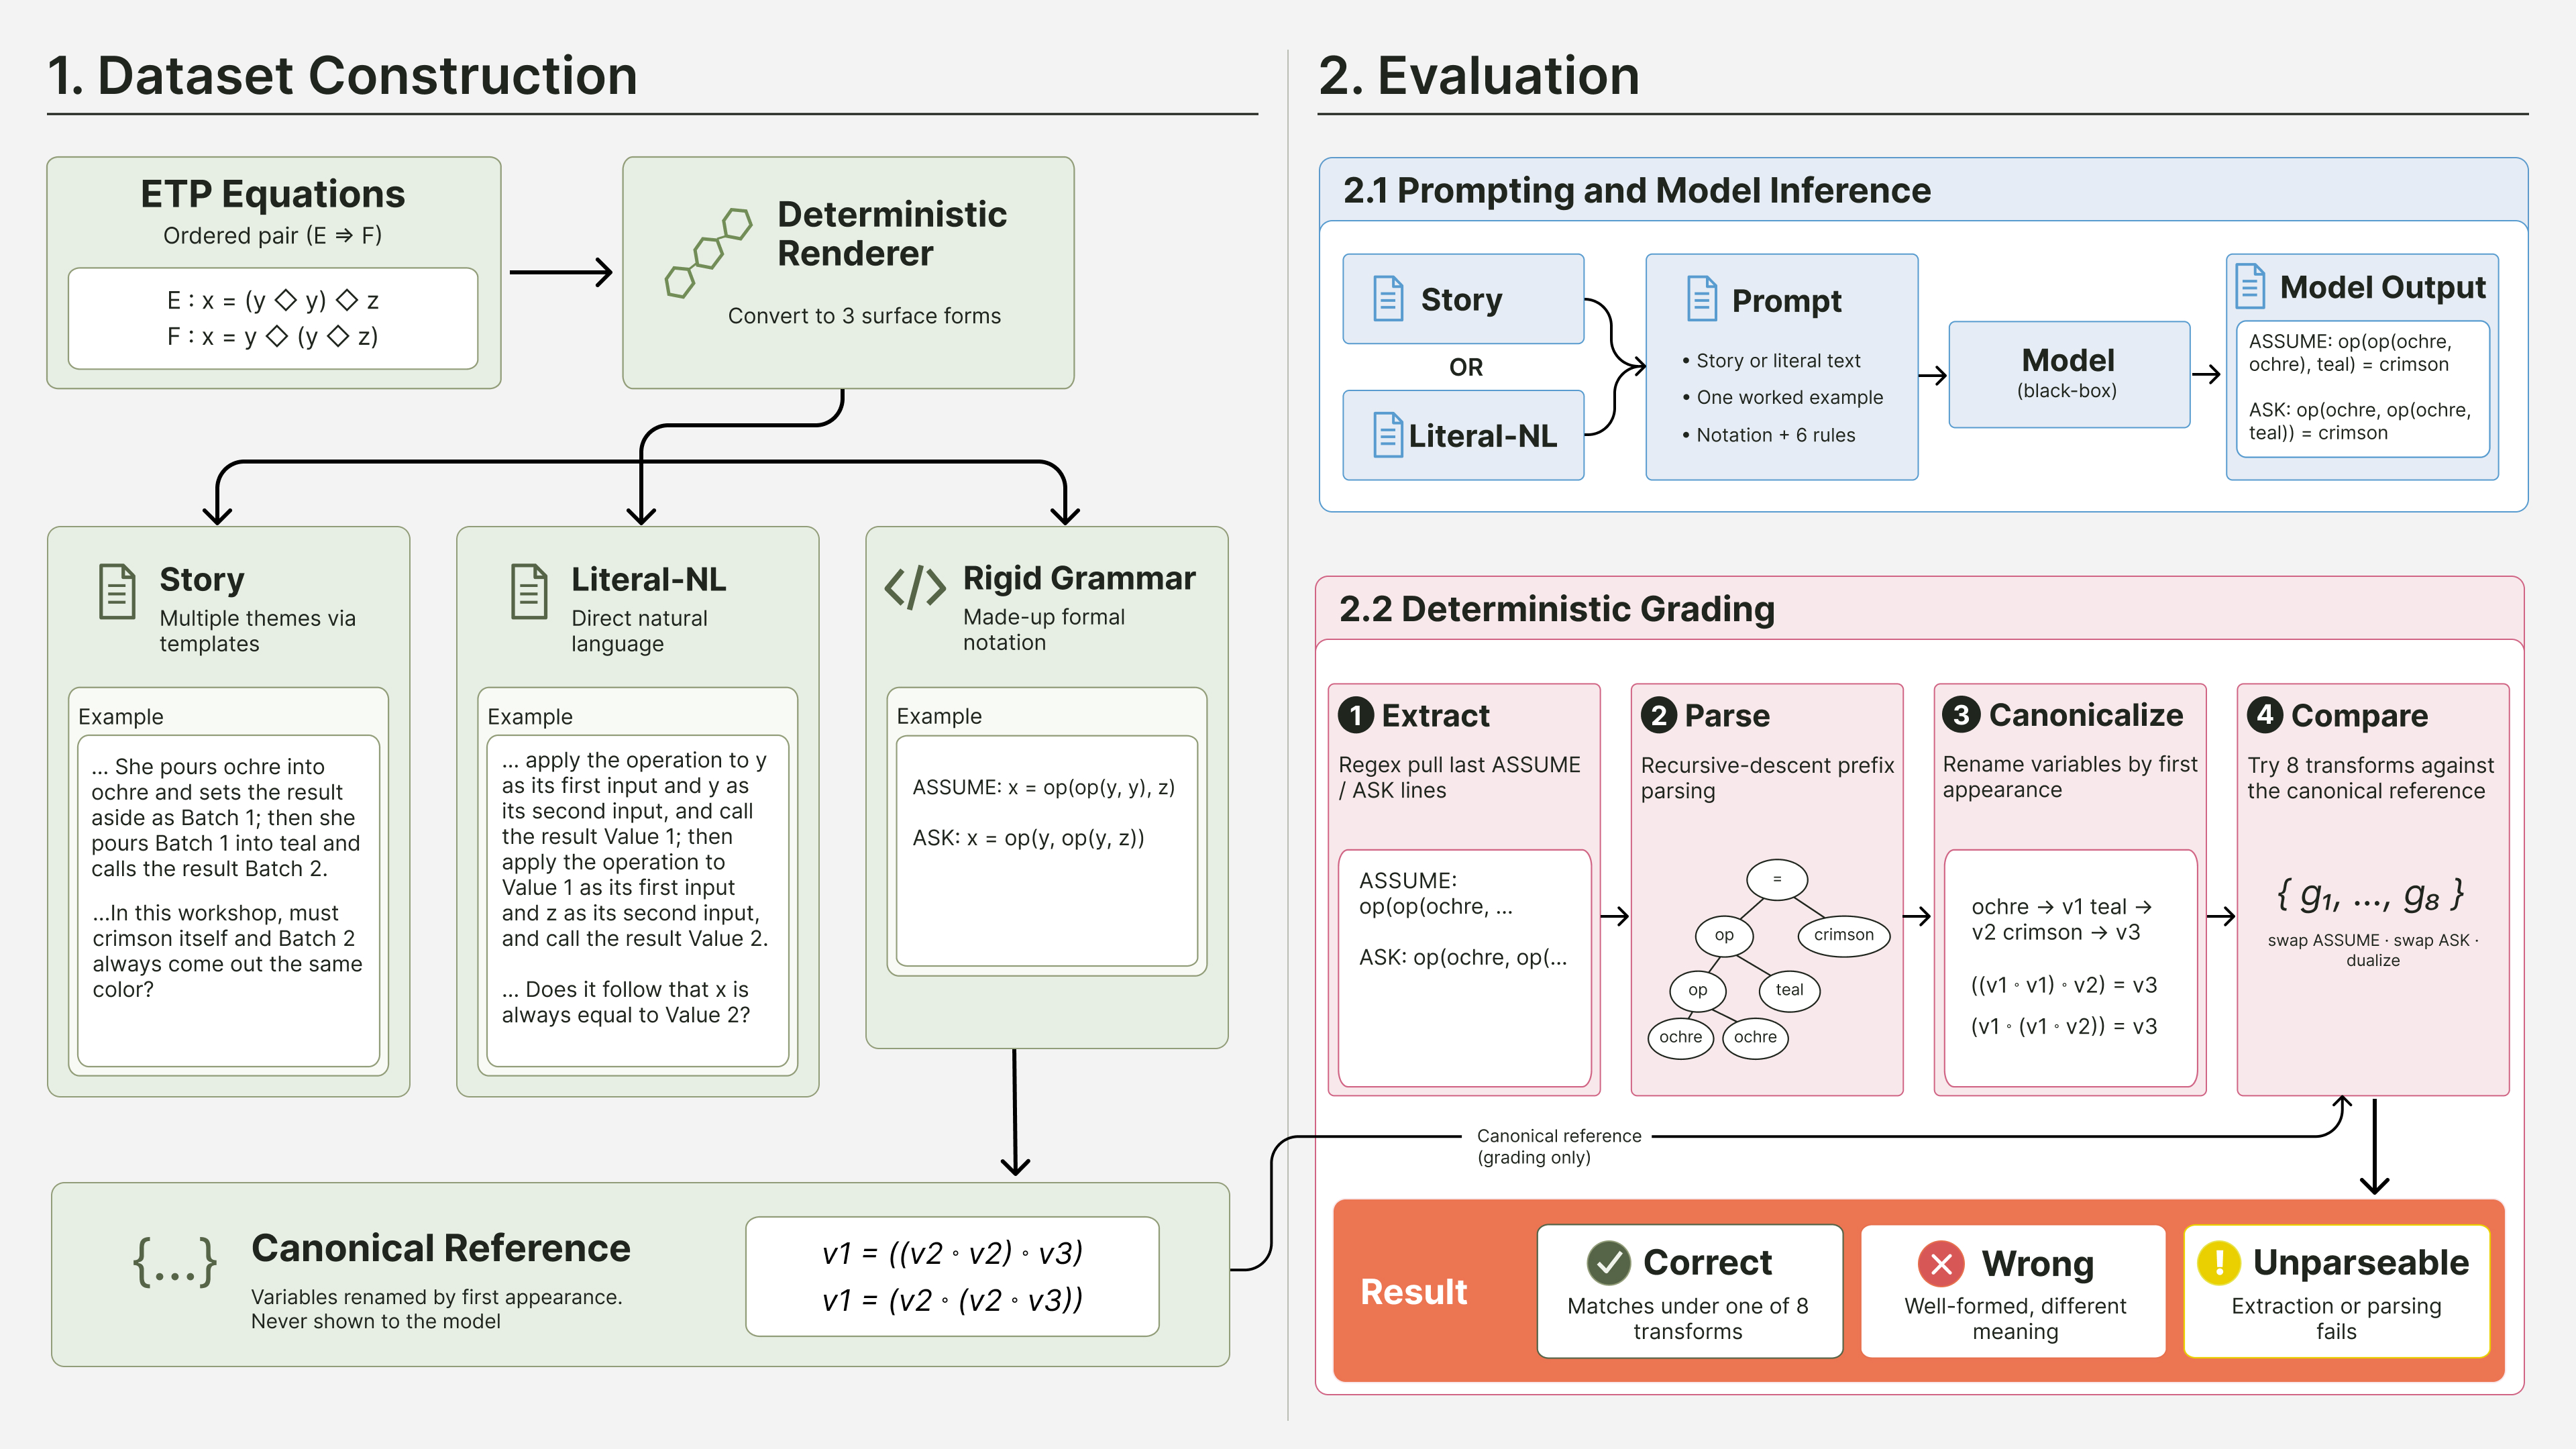
\includegraphics[width=\linewidth]{main-figure.jpg}
    \caption{\textbf{Benchmark pipeline.} Starting from an ETP implication, deterministic renderers produce matched Story and Literal-NL inputs. A model translates one input into Rigid Grammar, and a deterministic grader compares the parsed response with the retained formal source.}
  \label{fig:pipeline}
\end{figure}

\subsection{Substrate: implications between equational laws}
A \textit{magma} is a set equipped with a single binary operation
$\diamond$. A \textit{law} is a universally quantified
identity between terms of that operation, such as
$x \diamond y = (y \diamond y) \diamond x$;  The Equational Theories Project
catalogued the 4{,}694 laws with at most four applications of the operation
and resolved all 22{,}028{,}942 ordered implications between them, with the
complete graph verified in Lean [cite]. However, our benchmark is not concerned with the truth value of the implications. 
Three properties make this an unusually clean substrate for measuring
translation. First, equality of meaning is decidable: whether two answers
in this fragment state the same law is a small computation
(Section~\ref{sec:grading}), whereas for mathematics at large that question
can be as hard as the math itself. This is what lets the benchmark
dispense with judges. Second, difficulty is controllable and scales with the number of operation applications and the maximum
nesting depth. Third, the laws are uniform and obscure: beyond a handful
with established names (commutativity, associativity), they are nameless and
essentially absent from natural-language text, so a model cannot retrieve a
memorized formalization, it must read the story in front of it.
The two zero-operation laws ($x = x$ and
$x = y$) are excluded everywhere.\footnote{A law with no operation offers
nothing to translate, and models misread exactly these: they embellish the
trivial law by inventing an operation the text never states. Pairs
containing one also distort difficulty stratification, since all of the
pair's operations then sit in the partner law.}
\subsection{Informalization: rendering a statement as a story}
Figure~\ref{fig:benchmark-item} shows a complete item. The renderer maps
each law to a narrated procedure. Variables become ingredients from the
theme's fixed palette (crimson, ochre, \dots), assigned by order of first
appearance. Each application of the operation becomes one step of a
concrete, order-sensitive action, and every intermediate result is given a
name (``Batch 1''), so nesting is expressed by reference to earlier steps
rather than by nested prose. Universal quantification is narrated
explicitly (``take any two pigments at all,'' ``however she chooses'').
The assumed law $E$ is presented as an exceptionless custom of the
workplace; the questioned law $F$ is then posed as an open question,
quantified afresh, in one direction only, and left unanswered.
Four themes supply the vocabulary --- pouring pigments (\textit{paint}),
brewing over leaves (\textit{tea}), grafting cuttings (\textit{graft}),
relaying signals (\textit{signal}) --- while the sentence skeleton is
identical across them. Every
action phrasing is order-sensitive by design (``pours crimson \textit{into}
ochre''); symmetric wordings such as ``mix'' are banned, because they would
silently assert a commutativity the law may not have.
 
\subsection{The formalization task}
The prompt shown with each story is self-contained and defines the entire
target language on the page: an expression is an ingredient name or
$\mathtt{op}(\textit{first}, \textit{second})$, where \texttt{op} stands
for one performance of the story's combining action on its two inputs in a
fixed order; an equation asserts that two expressions always come out the
same; and the answer is exactly two lines,
\begin{quote}
\texttt{ASSUME: <equation for the custom that always holds>}\\
\texttt{ASK: <equation for the regularity the question asks about>}
\end{quote}
Its worked example uses a fifth setting (a bookbinder stacking volumes) that
never occurs in the corpus. Nothing about Lean, magmas, or the source
project is assumed or mentioned.
\subsection{Grading}
\label{sec:grading}
The grader extracts the last \texttt{ASSUME:} and \texttt{ASK:} lines from
the raw response and parses each in the tiny prefix grammar. If extraction
or parsing fails --- a missing line, malformed syntax, runaway nesting ---
the verdict is \textit{unparseable}. Otherwise both equations are
canonicalized by renaming variables in order of first appearance, and the
answer is compared with the source pair under all eight combinations of
three commuting involutions:
\begin{itemize}
    \item swapping the two sides of the assumed equation;
    \item swapping the two sides of the asked equation;
    \item dualizing both equations, i.e.\ mirroring the argument order of
    every \texttt{op} application.
\end{itemize}
The answer is \textit{correct} if some combination maps it onto the source
pair, and the minimal matching transform is recorded with the verdict, so
exact-convention answers remain distinguishable from swapped or dualized
ones.
Each accepted symmetry is a faithful reading of the story.
Ingredient names are arbitrary labels. ``Batch 1 and Batch 3 always come
out the same color'' is symmetric, so the order of an equation's sides is
not recoverable intent. And the story cannot say which participant of
``pours crimson into ochre'' is the operation's \textit{first} argument; an
answer that adopts the opposite convention uniformly states the dual law
--- the same claim with every application mirrored. However, any
structural difference makes the answer \textit{wrong}.
\textit{Wrong} is the verdict of interest: a well-formed answer denoting a
different statement is semantic drift. Keeping \textit{unparseable} separate matters because
the failures differ in kind: a model that does not understand the output format
is not the same as a model that writes fluent formal syntax meaning the
wrong thing.
\begin{figure}[t]
\centering
\fbox{\begin{minipage}{0.94\columnwidth}\small
\textit{In a certain paint workshop, the colorist follows one unbreakable
habit. Take any two pigments at all --- call the first crimson and the
second ochre. She runs two procedures side by side.}
\smallskip
\textit{In the first, she pours crimson into ochre and sets the result
aside as Batch 1.}
\smallskip
\textit{In the second, she pours ochre into ochre and calls the result
Batch 2; then she pours Batch 2 into crimson and calls that Batch 3.}
\smallskip
\textit{However she chooses her two starting pigments, Batch 1 and Batch 3
always come out the exact same color. That is simply how this workshop
works, without exception.}
\smallskip
\textit{One morning her apprentice wonders about something. Take any two
pigments --- again call the first crimson and the second ochre. Pour
crimson into ochre and set the result aside as Batch 1. Separately, pour
ochre into crimson and call the result Batch 2.}
\smallskip
\textit{In this workshop, must Batch 1 and Batch 2 always come out the same
color?}
\medskip
\hrule
\medskip
A correct answer, in the notation defined by the prompt:
\\
\texttt{ASSUME: op(crimson, ochre) = op(op(ochre, ochre), crimson)}\\
\texttt{ASK: op(crimson, ochre) = op(ochre, crimson)}
\end{minipage}}
\caption{One benchmark item. The renderer maps the implication
$x \diamond y = (y \diamond y) \diamond x \;\Rightarrow\;
x \diamond y = y \diamond x$ (ETP equations 387 and 43) to this story under
the \textit{paint} theme.}
\label{fig:benchmark-item}
\end{figure}
\subsection{A second rendering: Literal-NL}
Every pair can also be rendered by a second deterministic renderer that
omits the narrative flourish. The \textit{Literal-NL} arm produces a direct description
that openly speaks of an operation with a first and a second input and uses
letters for the objects, with the same one-step-per-application discipline:
``apply the operation to $x$ as its first input and $y$ as its second
input, and call the result Value 1; then \dots''. The description is
question-framed like the story and graded by the same grader.\footnote{On the literal arm
the text does fix which input is first, so a dualized answer is not a
faithful reading of \textit{this} text; the grader accepts and records it
anyway so that both arms are scored identically. Dualized answers are rare
in practice.}
The literal arm is the benchmark's built-in control. Sampling never
consults the rendering, so a story run and a literal run with the same seed
evaluate the identical pairs, and the gap between them isolates the cost of
the narrative indirection. The literal description is also, by
construction, what a perfect abstraction of the story would produce, which
is why it serves as the approximate ceiling for the two-stage protocol
studied in Section~\ref{sec:results}.

\subsection{Difficulty, sampling, and scale}
Two structural dials set item difficulty: the total number of operation
applications in the pair (two to eight, once the zero-operation laws are
excluded) and the maximum nesting depth of any term (one to four). Because
law counts grow rapidly with size, uniform sampling is dominated by
maximal four-plus-four-application pairs; benchmark samples are therefore
stratified, drawing a fixed number of pairs per total-operation bin with a
seeded deterministic sampler, so any run's instance set is reproducible
from its seed and equal seeds give identical pair sets across arms.
The substrate is effectively inexhaustible: the 4{,}694 laws yield roughly
22 million ordered pairs, each renderable under four themes, and a seeded
synthetic generator can produce laws beyond the four-application cap in the
same format when a longer difficulty axis is needed. This bears directly on
contamination. The stories are novel text that exists nowhere outside the
benchmark; the mapping from story to statement appears in no training
corpus. The marginal cost of an item is one model call, rendering and grading are free.

\section{Results}
\label{sec:results}
\subsection{Abstraction helps improve translation accuracy}
Rendering ETP mathematical statements as  stories rather than literal descriptions introduces a significant loss in auto-formalization faithfulness. Across nine models tested on a fixed 160-pair set, models correctly recovered statements from stories only $50\%$ of the time, compared to $67\%$ for literal descriptions (Figure~\ref{fig:surface-form}). Both start from identical pairs and undergo identical grading, attributing this disparity to the statement surface form. Notably, we see a bigger gap in the mid-sized open models, between $20$--$30$ points, as opposed to more capable models, where they are more resilient across formats.

Under the two-stage protocol, we prompt the model to abstract the problem before formalizing, where it first strips away the narrative to produce a notation-free logical summary, and then translate into the target syntax. This intermediate step recovers a median of $99\%$ of the story-to-literal performance drop, boosting the pooled story accuracy to $66\%$, effectively matching the literal baseline. This suggests the failure mode that models struggle to identify the core logical claim in a decorated narrative, but are able to translate more faithfully once the claim is isolated.


\begin{figure}[t]
\centering
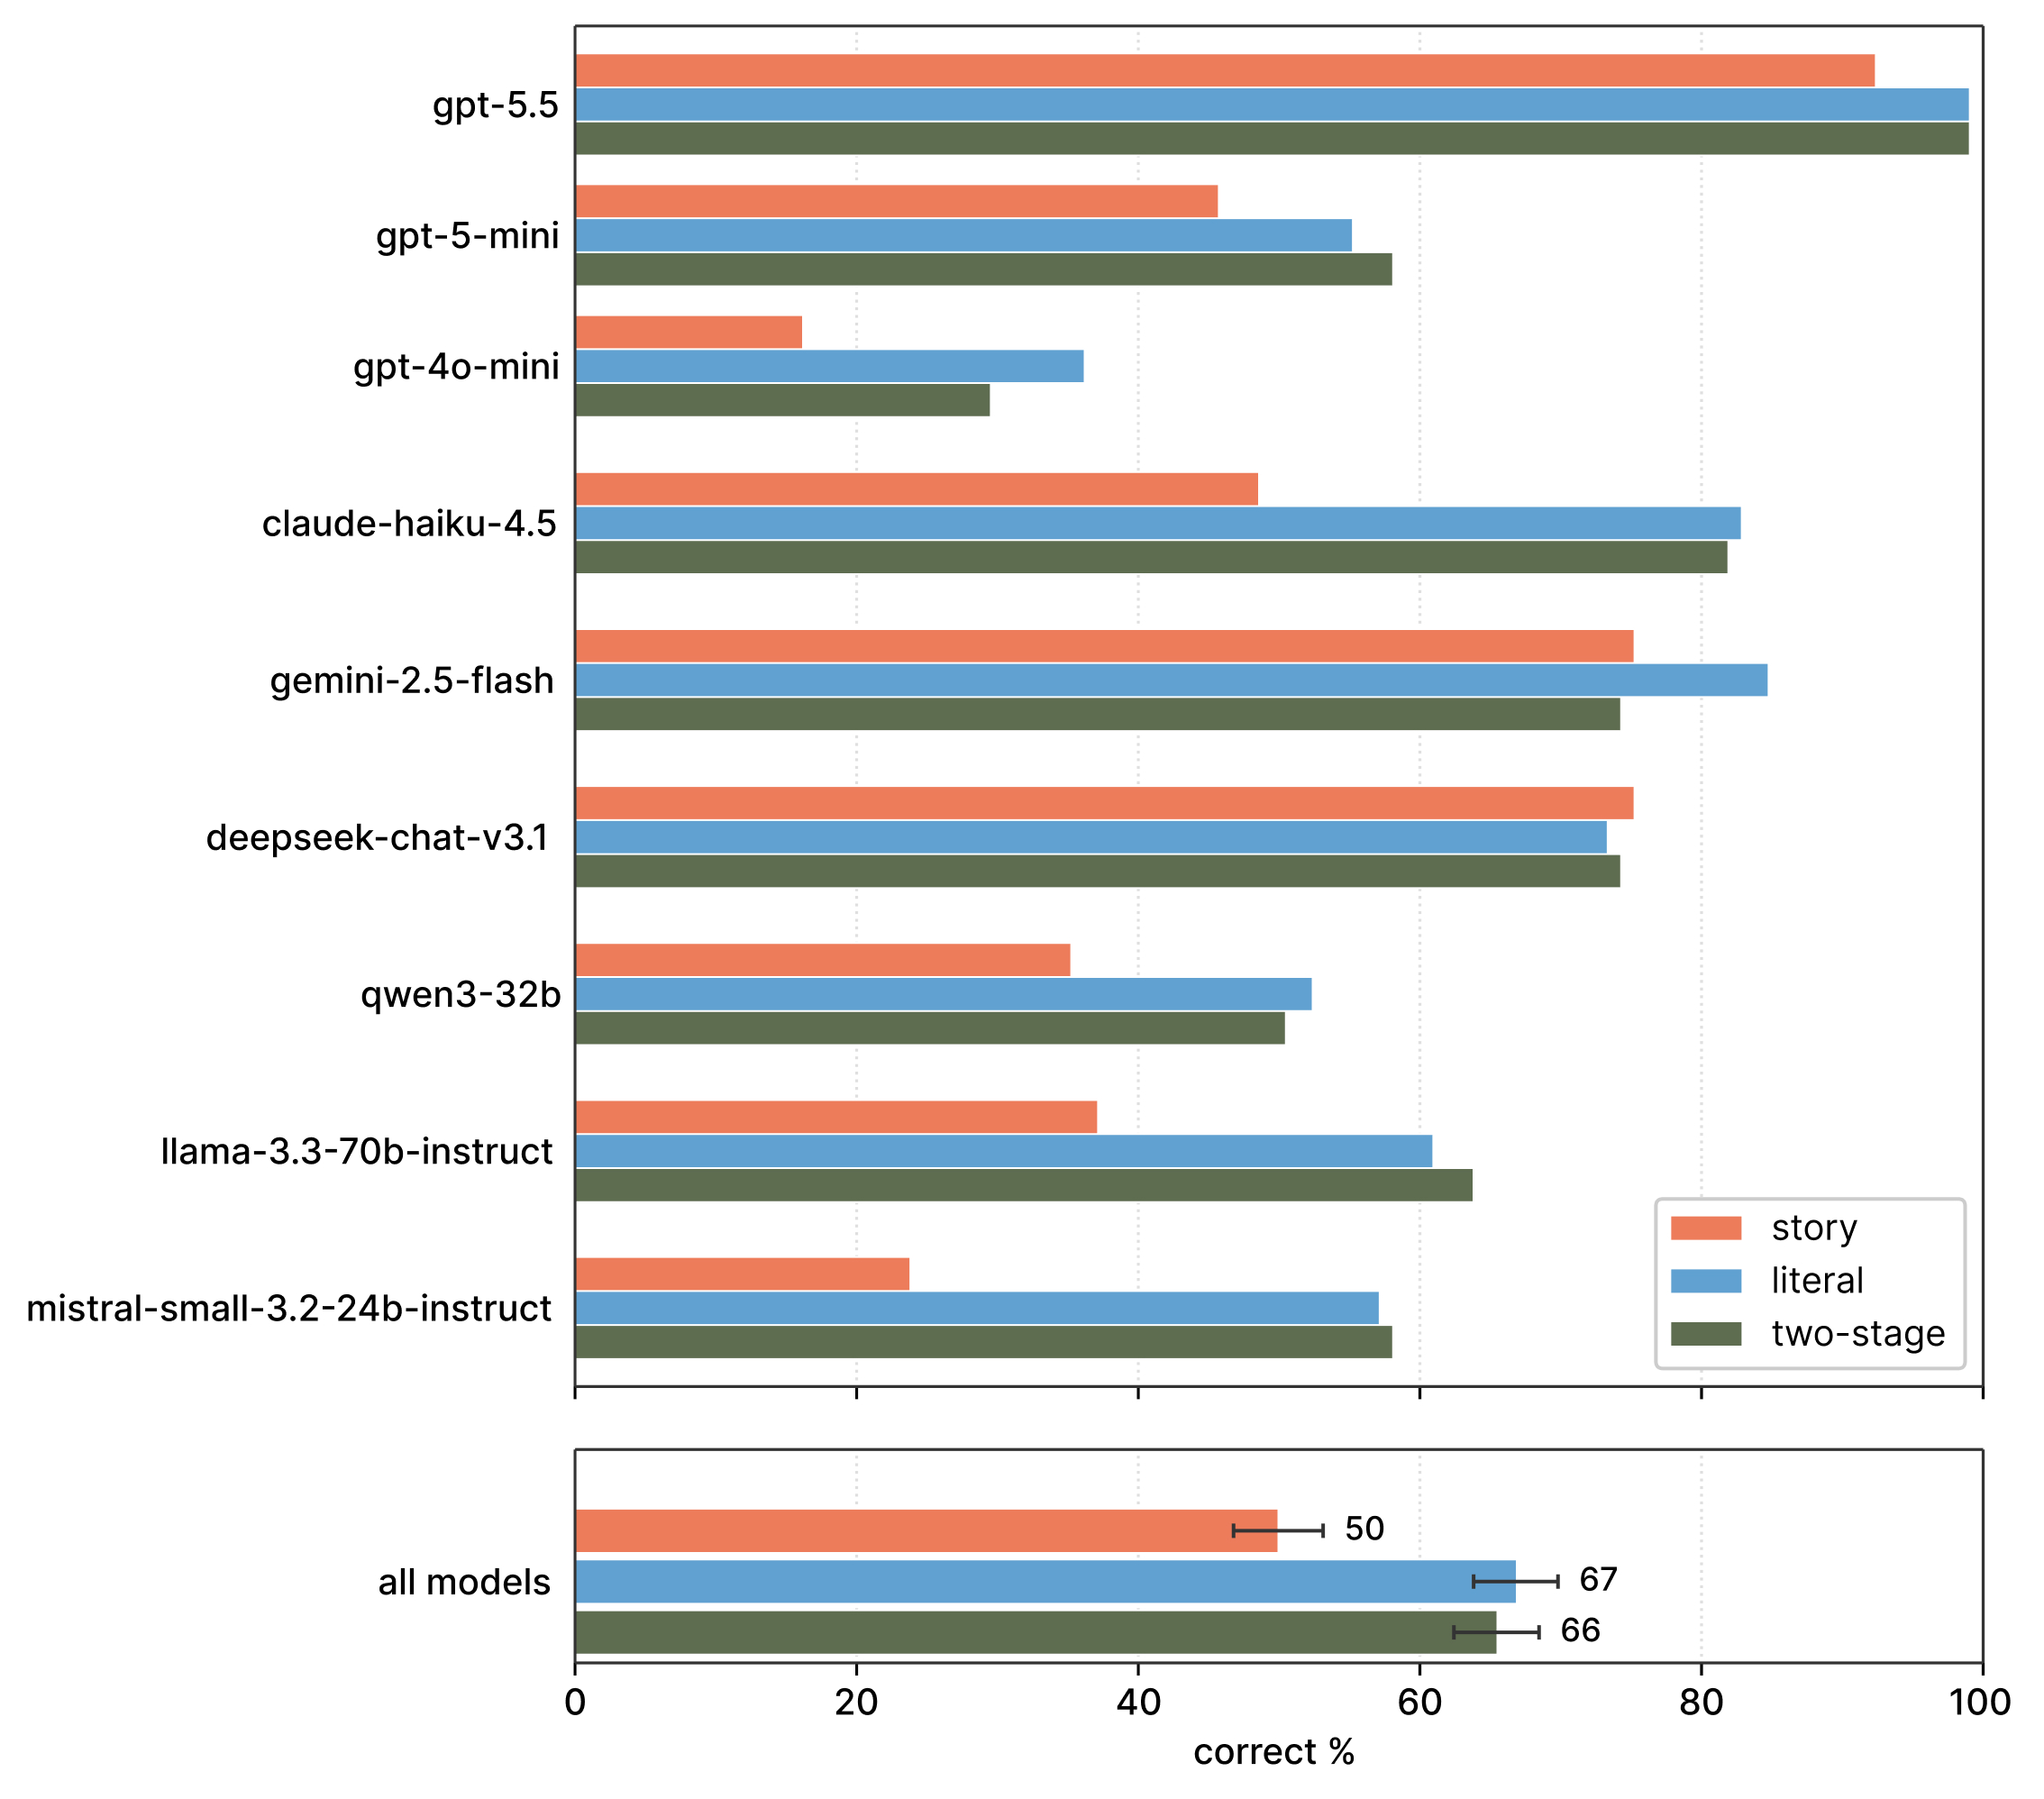
\includegraphics[width=0.85\columnwidth, height=0.38\textheight, keepaspectratio]{f2_arms_by_model-newer.jpg}
\caption{ Faithfulness by surface form, per model (nine models, 160
stratified pairs, no reasoning, vacuous laws excluded). 
 Story accuracy trails
literal accuracy for nearly every model; the two-stage protocol, which inserts one
abstraction step before formalizing, tracks the literal ceiling. The bottom
panel pools all models and pairs ($n = 945$ per surface form); error bars
are Wilson 95\% intervals.}
\label{fig:surface-form}
\end{figure}

\subsection{Reasoning significantly improves translation accuracy}
When reasoning capabilities are enabled, translation accuracy improves substantially across all three surface forms to near-ceiling levels. Notably, the narrative penalty plays a much smaller role when there is more compute, as we see that most of the models still reach near perfect translation accuracy from story surface form. Evaluating a matched set of pairs across eight models, story accuracy surges from $40\%$ to $97\%$, literal accuracy from $62\%$ to $99\%$, and two-stage accuracy from $59\%$ to $96\%$ (Figure~\ref{fig:reasoning}). The explicit benefits of the two-stage pipeline are subsumed when a model is allowed to perform that abstraction internally via extended deliberation.

\begin{figure}[H]
\centering
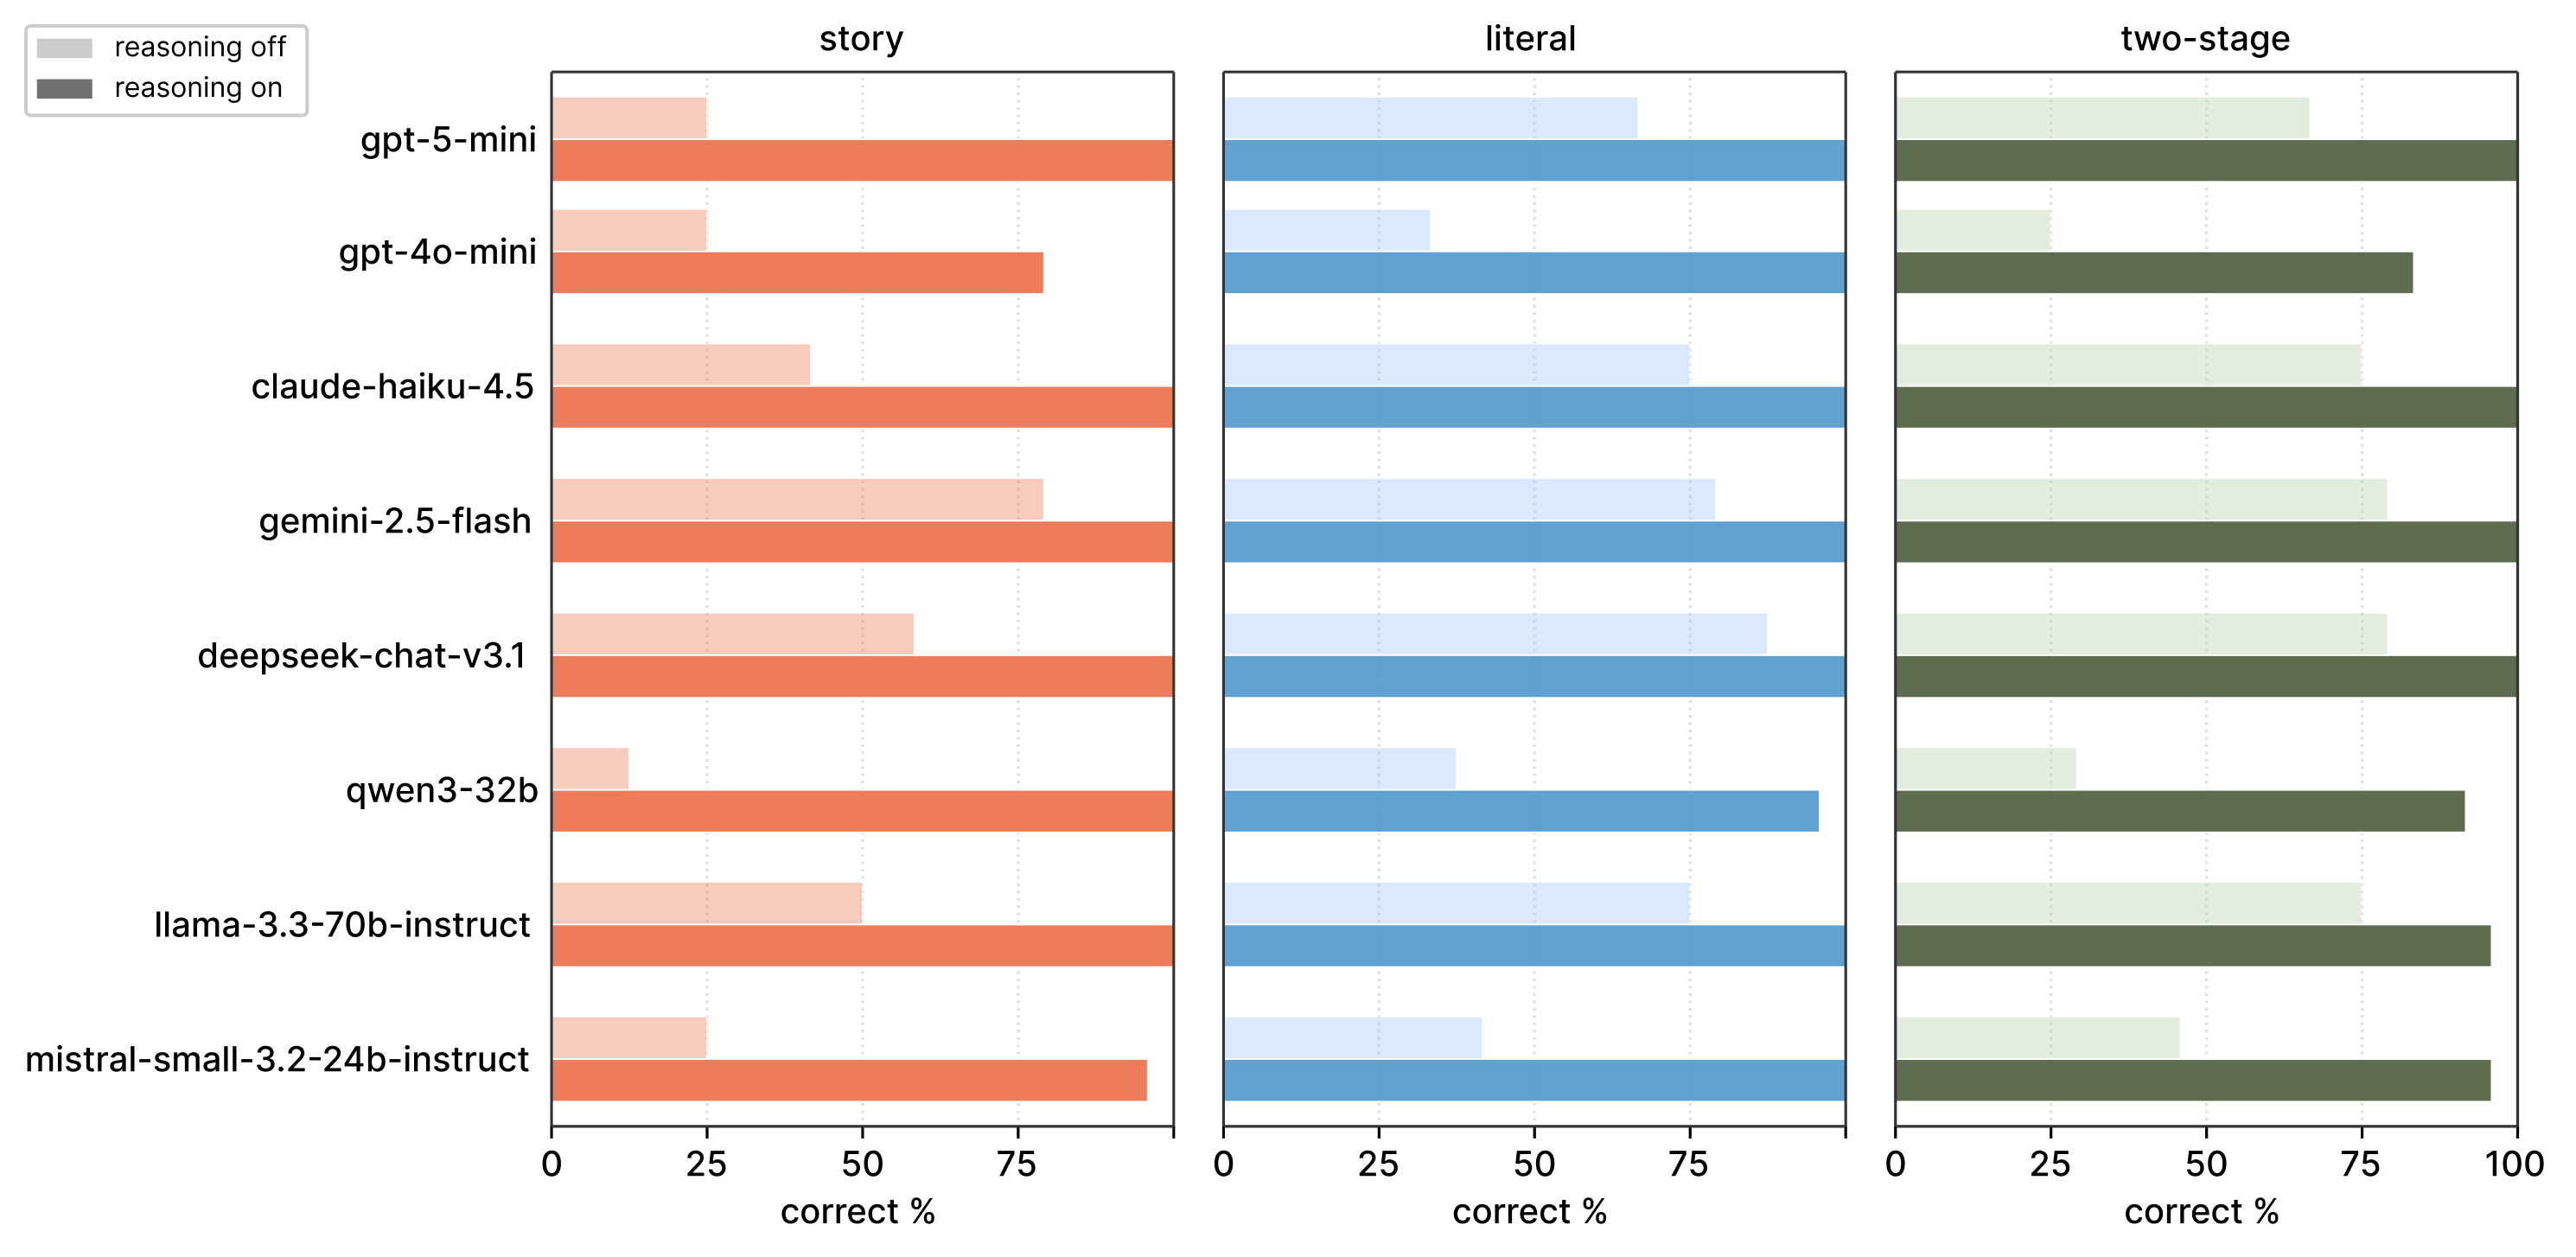
\includegraphics[width=\columnwidth, height=0.32\textheight, keepaspectratio]{r2_bars_by_model-newer.jpg}
% \caption{\shivam{You'd want to be consistent in the color scheme, throughout. Also if this barplot is vertical, then figure 1 should also be vertical. I would suggest taking the bare plot (no labels and or legend) and use figma to size and place them better} \denis{done} Faithfulness with reasoning disabled (light) versus enabled (dark),
per model and surface form. Reasoning raises every surface form close to the ceiling and
largely removes the story penalty visible in Figure~\ref{fig:surface-form}.}
\label{fig:reasoning}
\end{figure}

Closing the gap is not free. Every reasoning-capable model spends more thinking tokens on a story than on the matched literal description of the same statement: between $1.1\times$ and $1.5\times$ as many at the median, with the strongest reasoners at the high end of that range (Appendix~\ref{app:tokens}, Table~\ref{tab:tokens}). \shivam{what is a token multiplier? If the point is to that that the models use 1.4-1.5x tokens, then just say that} \denis{done} The model has to spend additional inference-time compute to extract the formal structure from the unstructured narrative before it can translate it. \shivam{Again, too jargony text. You'd want to write some the model need to spend significant inference-time compute to extract the formal structure from the noisy, unstructured natural language.} \denis{done} \shivam{This result also looks trivial, one would expect more token usage for the reasoning model, and more complex task, it should be moved to appendix in favor ouf other results.} \denis{done}

\subsection{Reasoning tokens scale with translation task complexity}

To test how faithfulness holds up on harder statements, we extended our difficulty axis beyond the Equational Theories Project (ETP) limit of four operations, generating synthetic laws with up to ten operations per equation. Without reasoning, accuracy collapses as complexity grows, dropping from $82\%$ at one operation per equation to $0\%$ at ten on the story form. With reasoning enabled, the same five models degrade gracefully and still recover $75\%$ to $81\%$ of statements at the hardest tier (Figure~\ref{fig:cliff}). Their reasoning effort scales with the task: median thinking tokens rise monotonically with operation count, and stories cost more than literal descriptions at every level, with the gap widening as statements get harder (Appendix~\ref{app:tokens}, Figure~\ref{fig:tokens-complexity}). Taken together, the steep cliff seen without reasoning is consistent with a deliberation-budget constraint rather than a representational limit: given room to think, models allocate more compute to harder statements and maintain semantic faithfulness.

\begin{figure}[H]
\centering
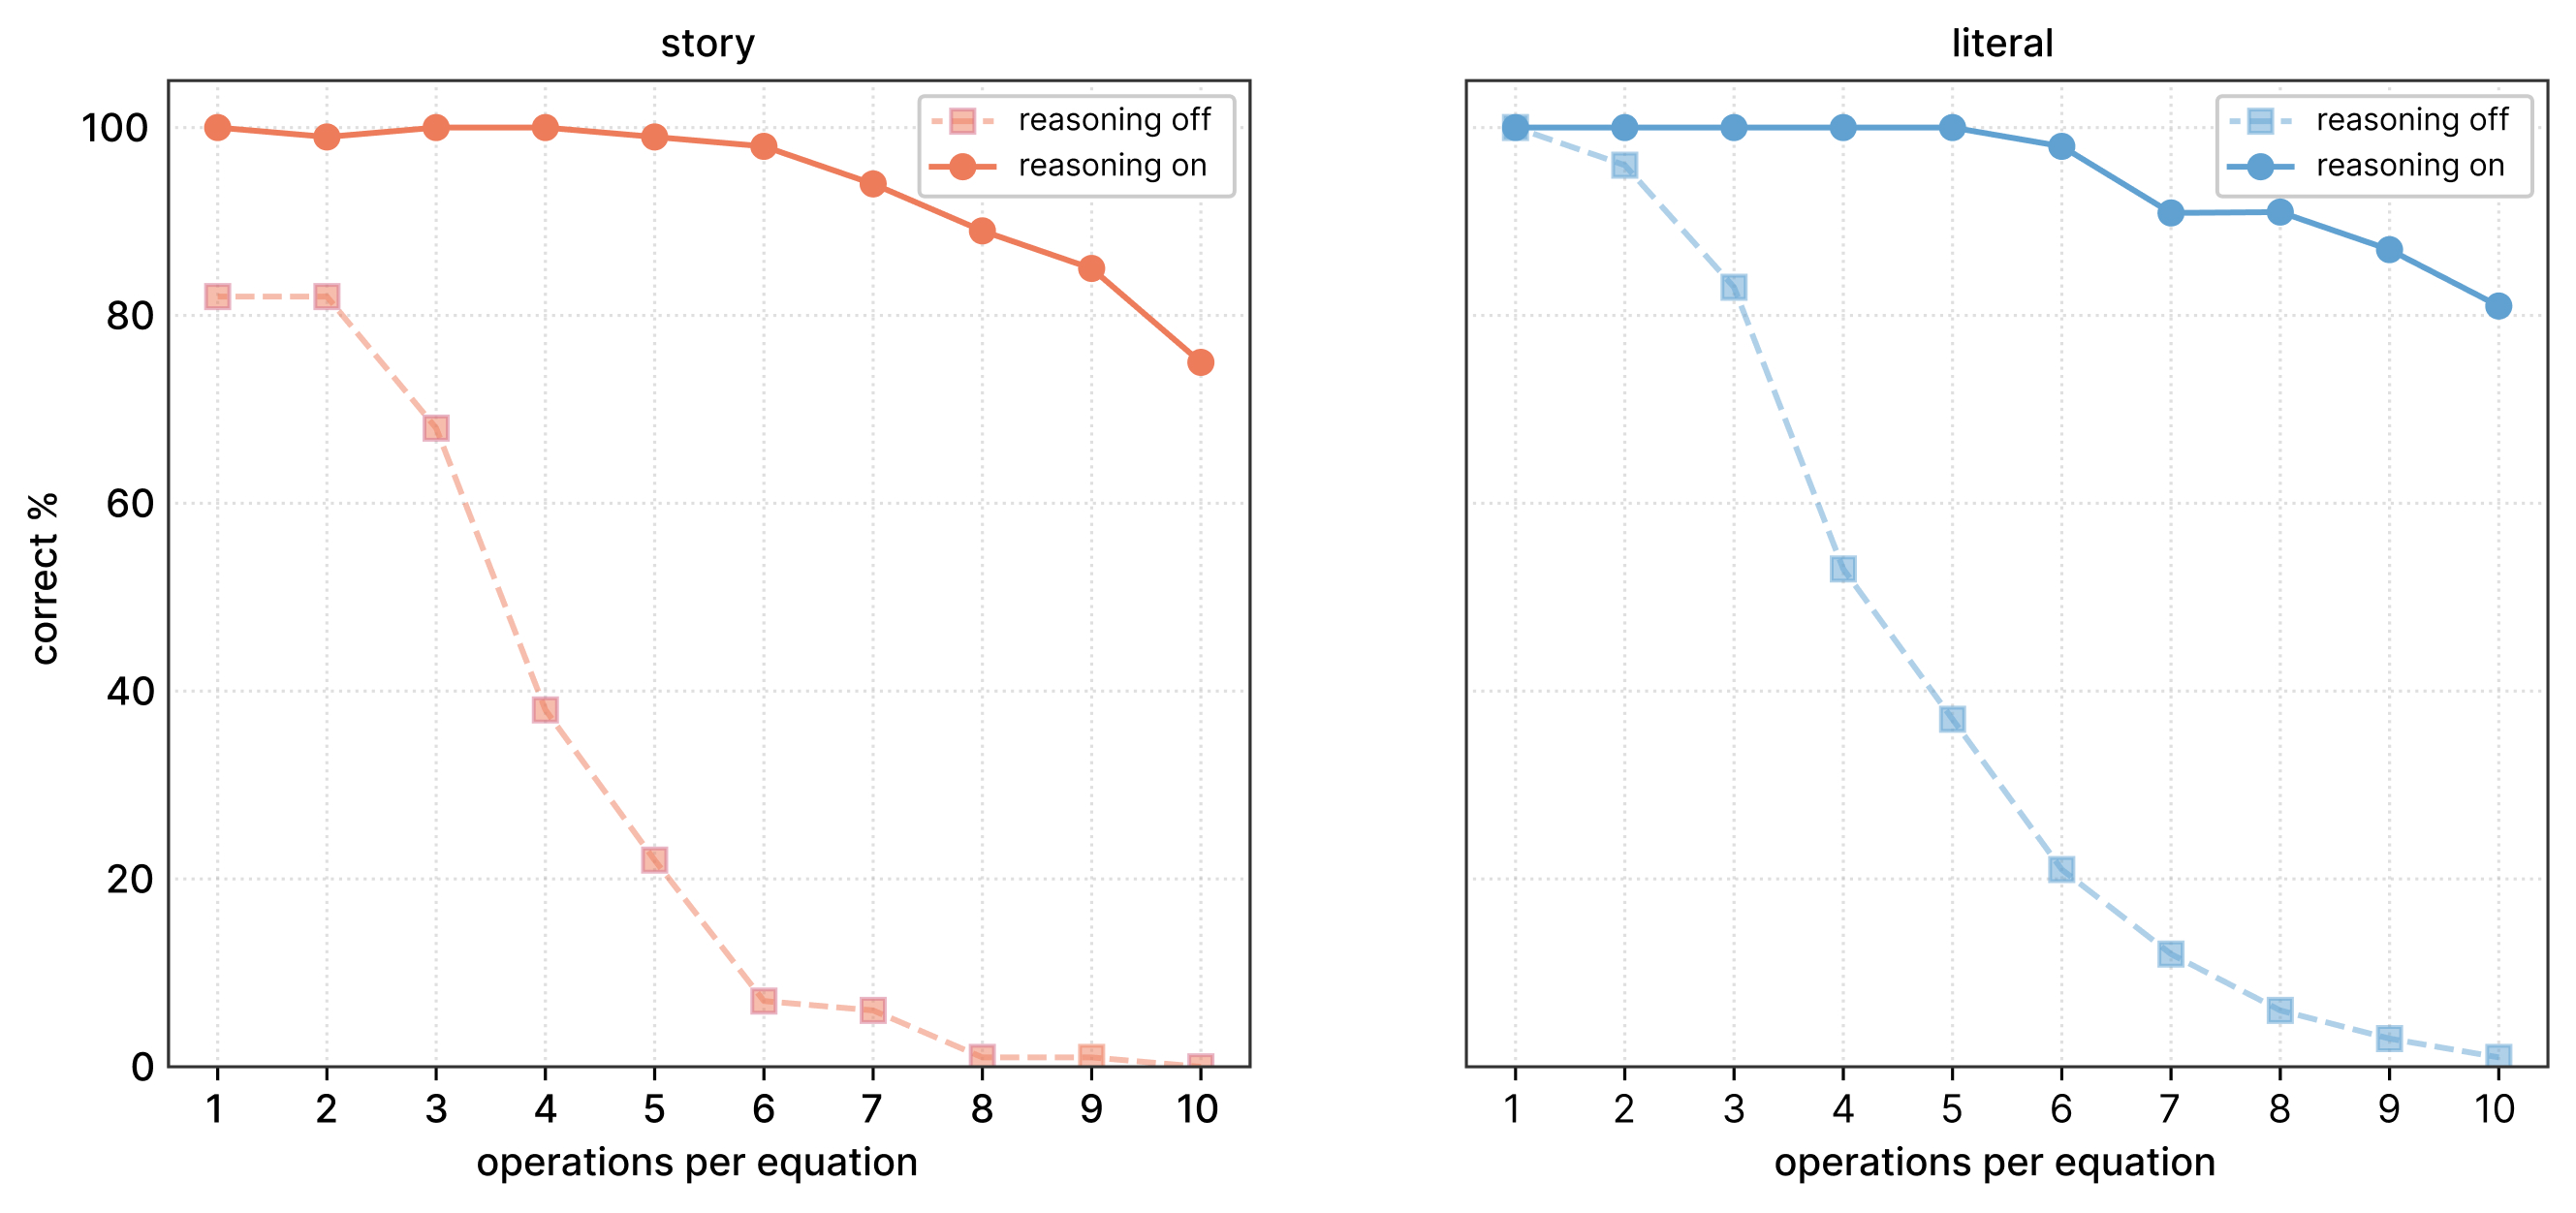
\includegraphics[width=\columnwidth]{accuracy_on_vs_off-new.jpg}
\caption{Faithfulness against complexity with reasoning disabled versus
enabled. Without reasoning, accuracy cliffs toward zero as complexity grows;
with reasoning, both surface forms degrade gracefully, indicating that the cliff is
chiefly a matter of deliberation budget rather than a representational limit.}
\label{fig:cliff}
\end{figure}

\section{Limitations}
Our benchmark deliberately studies a restricted form of autoformalization.
The natural-language inputs are generated from formal statements using fixed,
information-preserving templates. This construction provides exact ground
truth, but it reverses the direction in which real autoformalization datasets
are usually created and avoids much of the ambiguity found in human-written
mathematics. The four Story themes also share a common underlying structure,
so they capture narrative variation rather than the full linguistic diversity
of natural language.

The target rigid grammar represents equations over a single binary operation.
Its simplicity helps reduce target-language confounds, but it does not include
the types, notation, library dependencies, or elaboration behavior of practical
formal systems such as Lean. Our results therefore measure whether models
recover a controlled logical structure, not whether they can formalize
general mathematical statements or construct proofs. Deterministic grading is
exact only relative to the benchmark's representation and accepted
symmetries.

Finally, the strongest models approach ceiling performance under reasoning,
which limits the benchmark's ability to distinguish among frontier systems at
the current difficulty levels. Extending the structural complexity and
linguistic variation may reduce this saturation, but doing so while preserving
deterministic and unambiguous grading remains an important design challenge.


\section{Conclusion}
We introduced a controlled benchmark for studying semantic preservation in
natural-language-to-formal translation. Starting from ETP implications, we
generate matched Story and Literal-NL descriptions and ask models to recover
the same statement in a minimal rigid grammar. Because the original formal
statement is retained, model outputs can be graded deterministically without
a human or language-model judge.

Our paired evaluation shows that narrative presentation makes formalization
more difficult than a direct natural-language description of the same logical
structure. When reasoning is disabled, an explicit two-stage procedure recovers
most of this gap. When reasoning is enabled, all three conditions approach
ceiling performance, suggesting that additional inference-time computation
can allow capable models to perform the abstraction internally.

These results show that source interpretation and target encoding should be
treated as distinct components of autoformalization. The present benchmark
provides a controlled environment for studying their interaction rather than
a general solution to semantic faithfulness. A natural next step is to extend
this framework toward less templated language and richer target formalisms,
while retaining a reliable reference against which semantic drift can be
measured.

% \section*{References}


\bibliographystyle{plainnat}
\bibliography{references}


%%%%%%%%%%%%%%%%%%%%%%%%%%%%%%%%%%%%%%%%%%%%%%%%%%%%%%%%%%%%

\appendix

\section{Reasoning-token costs}
\label{app:tokens}

Table~\ref{tab:tokens} reports median reasoning tokens per item for the five
reasoning-capable models on the matched pairs of Section~\ref{sec:results},
with reasoning enabled. Every model spends more on the story than on the
literal description of the same statement. Figure~\ref{fig:tokens-complexity}
shows the same quantity against statement complexity on the synthetic laws of
one to ten operations per equation.

\begin{table}[H]
\centering
\caption{Median reasoning tokens spent per item on matched pairs, with
reasoning enabled (five reasoning-capable models). Each model consistently
deliberates more on the story than on the equivalent literal description.}
\label{tab:tokens}
\begin{tabular}{lccc}
\toprule
model & story & literal & ratio \\
\midrule
deepseek-chat-v3.1 & 1030 & 925 & 1.11 \\
claude-haiku-4.5 & 682 & 572 & 1.19 \\
qwen3-32b & 1046 & 733 & 1.43 \\
gemini-2.5-flash & 2116 & 1434 & 1.48 \\
gpt-5-mini & 1248 & 832 & 1.50 \\
\bottomrule
\end{tabular}
\end{table}

\denis{need to fix Figure 5, consider only keeping the 2 main lines}

\begin{figure}[H]
\centering
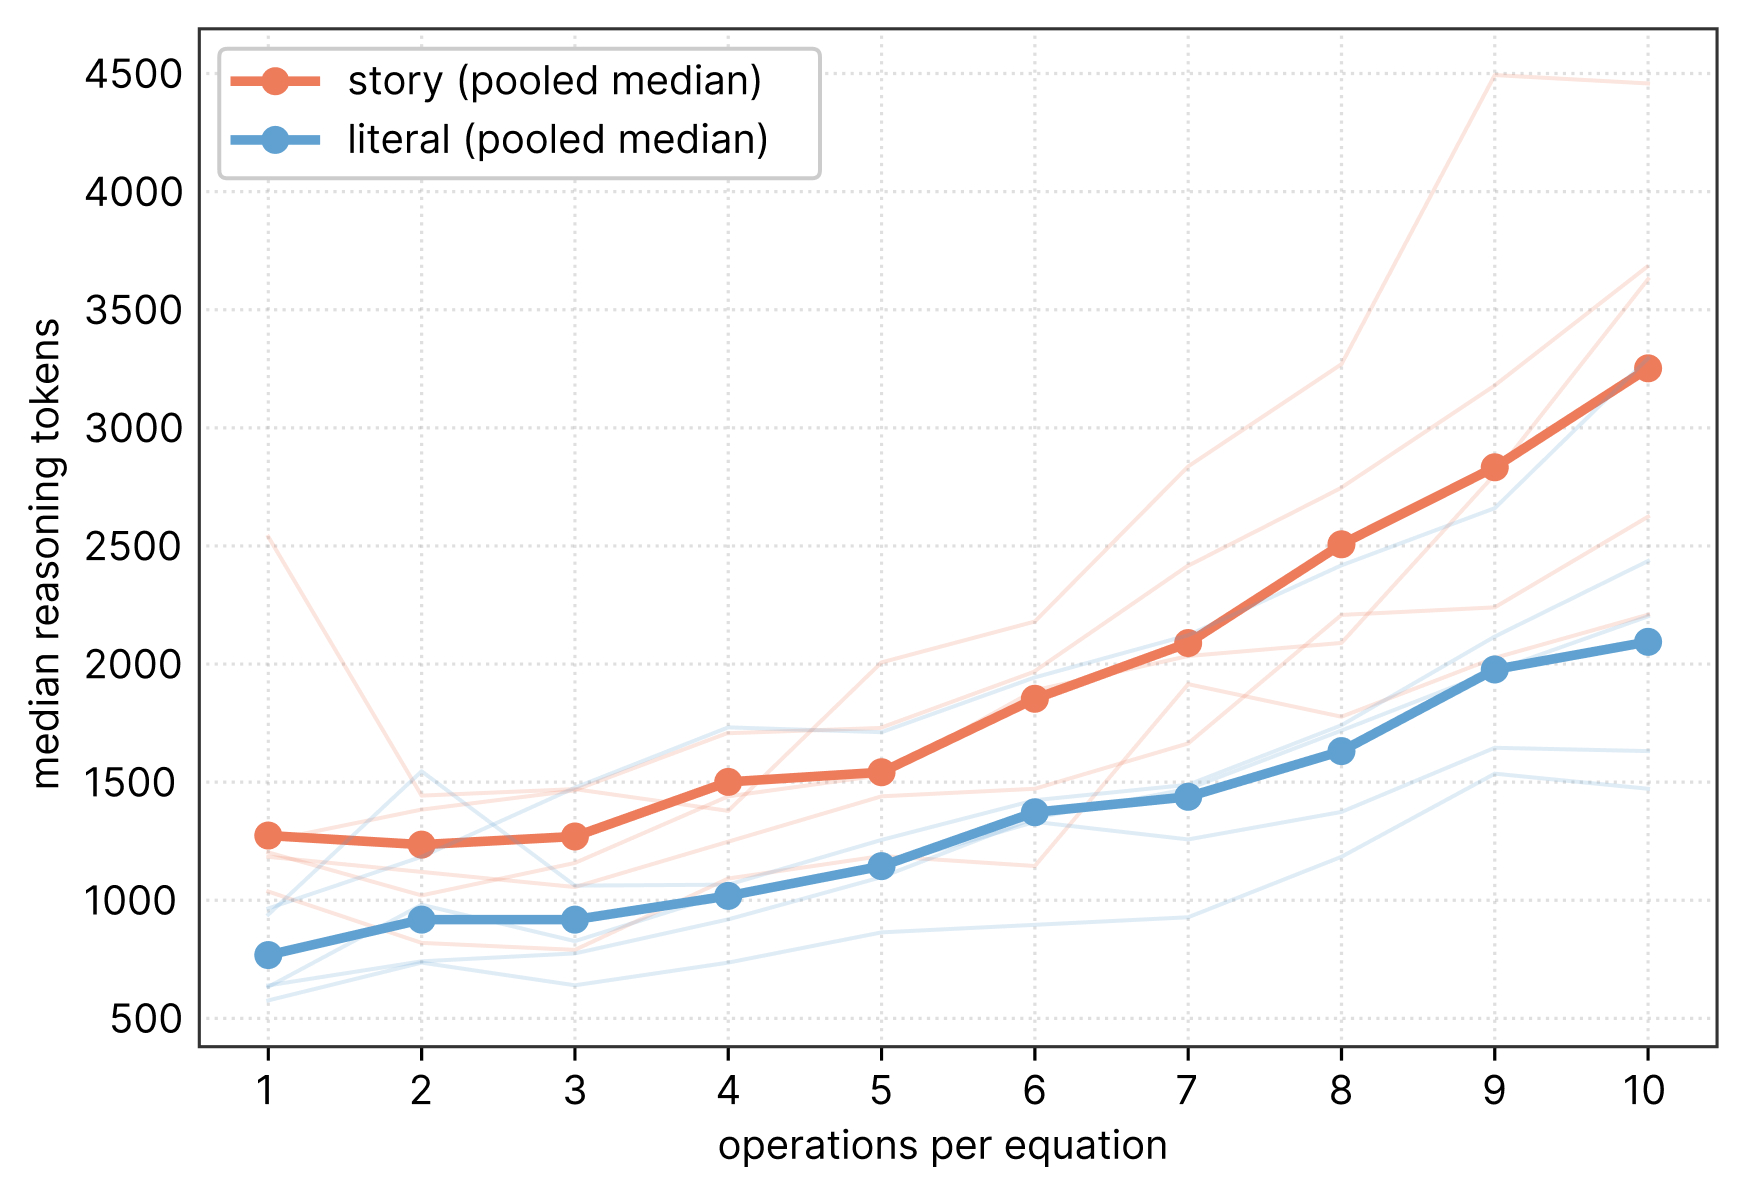
\includegraphics[width=0.7\columnwidth]{tokens_vs_complexity-new.jpg}
\caption{Median reasoning tokens per item against statement complexity (five
reasoning-capable models, synthetic laws of one to ten operations per
equation, reasoning enabled). Bold lines are pooled medians, faint lines are
individual models. Effort rises monotonically with complexity, and stories
cost more than the matched literal descriptions throughout.}
\label{fig:tokens-complexity}
\end{figure}

%%%%%%%%%%%%%%%%%%%%%%%%%%%%%%%%%%%%%%%%%%%%%%%%%%%%%%%%%%%%

\newpage
\input{checklist.tex}


\end{document}